\chapter{Tree algorithms}

\index{tree}

A \key{tree} is a connected, acyclic graph
that consists of $n$ nodes and $n-1$ edges.
Removing any edge from a tree divides it
into two components,
and adding any edge to a tree creates a cycle.
Moreover, there is always a unique path between any
two nodes of a tree.

For example, the following tree consists of 7 nodes and 6 edges:
\begin{center}
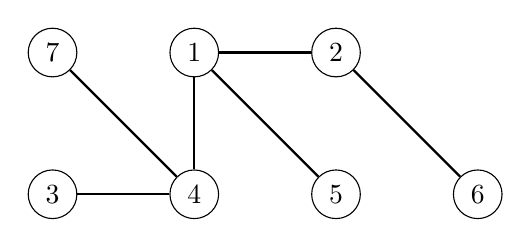
\begin{tikzpicture}[scale=0.9]
\node[draw, circle] (1) at (0,3) {$1$};
\node[draw, circle] (2) at (2,3) {$2$};
\node[draw, circle] (3) at (0,1) {$4$};
\node[draw, circle] (4) at (2,1) {$5$};
\node[draw, circle] (5) at (4,1) {$6$};
\node[draw, circle] (6) at (-2,3) {$7$};
\node[draw, circle] (7) at (-2,1) {$3$};
\path[draw,thick,-] (1) -- (2);
\path[draw,thick,-] (1) -- (3);
\path[draw,thick,-] (1) -- (4);
\path[draw,thick,-] (2) -- (5);
\path[draw,thick,-] (3) -- (6);
\path[draw,thick,-] (3) -- (7);
\end{tikzpicture}
\end{center}

\index{leaf}

The \key{leaves} of a tree are the nodes
with degree 1, i.e., with only one neighbor.
For example, the leaves of the above tree
are nodes 3, 5, 6 and 7.

\index{root}
\index{rooted tree}

In a \key{rooted} tree, one of the nodes
is appointed the \key{root} of the tree,
and all other nodes are
placed underneath the root.
For example, in the following tree,
node 1 is the root of the tree.

\begin{center}
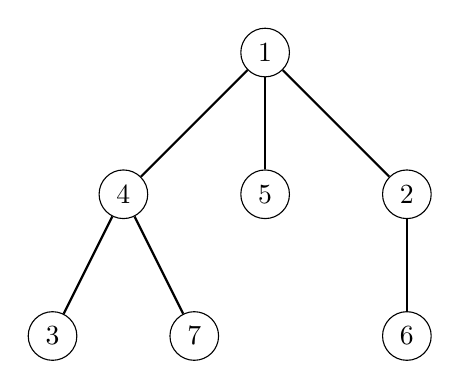
\begin{tikzpicture}[scale=0.9]
\node[draw, circle] (1) at (0,3) {$1$};
\node[draw, circle] (2) at (2,1) {$2$};
\node[draw, circle] (3) at (-2,1) {$4$};
\node[draw, circle] (4) at (0,1) {$5$};
\node[draw, circle] (5) at (2,-1) {$6$};
\node[draw, circle] (6) at (-3,-1) {$3$};
\node[draw, circle] (7) at (-1,-1) {$7$};
\path[draw,thick,-] (1) -- (2);
\path[draw,thick,-] (1) -- (3);
\path[draw,thick,-] (1) -- (4);
\path[draw,thick,-] (2) -- (5);
\path[draw,thick,-] (3) -- (6);
\path[draw,thick,-] (3) -- (7);
\end{tikzpicture}
\end{center}

\index{child}
\index{parent}

In a rooted tree, the \key{children} of a node
are its lower neighbors, and the \key{parent} of a node
is its upper neighbor.
Each node has exactly one parent,
except for the root that does not have a parent.
For example, in the above tree,
the children of node 4 are nodes 3 and 7,
and the parent is node 1.

\index{subtree}

The structure of a rooted tree is \emph{recursive}:
each node in the tree is the root of a \key{subtree}
that contains the node itself and all other nodes
that can be reached by traversing down the tree.
For example, in the above tree, the subtree of node 4
consists of nodes 4, 3 and 7.

\section{Tree traversal}

Depth-first search and breadth-first search
can be used for traversing the nodes in a tree.
The traversal of a tree is easier to implement than
that of a general graph, because
there are no cycles in the tree and it is not
possible to reach a node from multiple directions.

The typical way to traverse a tree is to start
a depth-first search at an arbitrary node.
The following recursive function can be used:

\begin{lstlisting}
void dfs(int s, int e) {
    // process node s
    for (auto u : adj[s]) {
        if (u != e) dfs(u, s);
    }
}
\end{lstlisting}

The function parameters are the current node $s$
and the previous node $e$.
The purpose of the parameter $e$ is to make sure
that the search only moves to nodes
that have not been visited yet.

The following function call starts the search
at node $x$:

\begin{lstlisting}
dfs(x, 0);
\end{lstlisting}

In the first call $e=0$, because there is no
previous node, and it is allowed
to proceed to any direction in the tree.

\subsubsection{Dynamic programming}

Dynamic programming can be used to calculate
some information during a tree traversal.
Using dynamic programming, we can, for example,
calculate in $O(n)$ time for each node
in a rooted tree the
number of nodes in its subtree
or the length of the longest path from the node
to a leaf.

As an example, let us calculate for each node $s$
a value $\texttt{count}[s]$: the number of nodes in its subtree.
The subtree contains the node itself and
all nodes in the subtrees of its children.
Thus, we can calculate the number of nodes
recursively using the following code:

\begin{lstlisting}
void dfs(int s, int e) {
    count[s] = 1;
    for (auto u : adj[s]) {
        if (u == e) continue;
        dfs(u, s);
        count[s] += count[u];
    }
}
\end{lstlisting}

\section{Diameter}

\index{diameter}

The \key{diameter} of a tree
is the length of the longest path
between two nodes in the tree.
For example, in the tree
\begin{center}
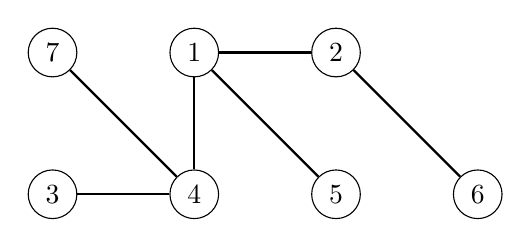
\begin{tikzpicture}[scale=0.9]
\node[draw, circle] (1) at (0,3) {$1$};
\node[draw, circle] (2) at (2,3) {$2$};
\node[draw, circle] (3) at (0,1) {$4$};
\node[draw, circle] (4) at (2,1) {$5$};
\node[draw, circle] (5) at (4,1) {$6$};
\node[draw, circle] (6) at (-2,3) {$7$};
\node[draw, circle] (7) at (-2,1) {$3$};
\path[draw,thick,-] (1) -- (2);
\path[draw,thick,-] (1) -- (3);
\path[draw,thick,-] (1) -- (4);
\path[draw,thick,-] (2) -- (5);
\path[draw,thick,-] (3) -- (6);
\path[draw,thick,-] (3) -- (7);
\end{tikzpicture}
\end{center}
the diameter is 4, and it corresponds to two paths:
the path between nodes 3 and 6,
and the path between nodes 7 and 6.

Next we will learn two efficient algorithms
for calculating the diameter of a tree.
Both algorithms calculate the diameter in $O(n)$ time.
The first algorithm is based on dynamic programming,
and the second algorithm uses two depth-first searches
to calculate the diameter.

\subsubsection{Algorithm 1}

First, we root the tree arbitrarily.
After this, we use dynamic programming
to calculate for each node $x$
the length of the longest path that begins at some leaf,
ascends to $x$ and then descends to another leaf.
The length of the
longest such path equals the diameter of the tree.

In the example graph, the longest path begins at node 7,
ascends to node 1, and then descends to node 6:
\begin{center}
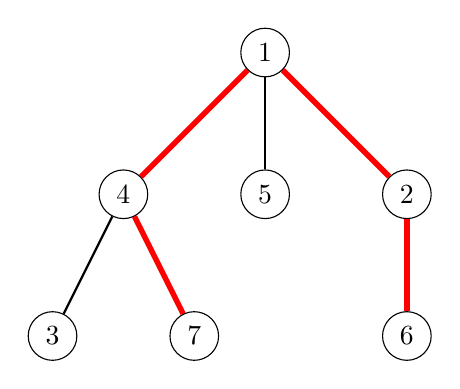
\begin{tikzpicture}[scale=0.9]
\node[draw, circle] (1) at (0,3) {$1$};
\node[draw, circle] (2) at (2,1) {$2$};
\node[draw, circle] (3) at (-2,1) {$4$};
\node[draw, circle] (4) at (0,1) {$5$};
\node[draw, circle] (5) at (2,-1) {$6$};
\node[draw, circle] (6) at (-3,-1) {$3$};
\node[draw, circle] (7) at (-1,-1) {$7$};
\path[draw,thick,-] (1) -- (2);
\path[draw,thick,-] (1) -- (3);
\path[draw,thick,-] (1) -- (4);
\path[draw,thick,-] (2) -- (5);
\path[draw,thick,-] (3) -- (6);
\path[draw,thick,-] (3) -- (7);

\path[draw,thick,-,color=red,line width=2pt] (7) -- (3);
\path[draw,thick,-,color=red,line width=2pt] (3) -- (1);
\path[draw,thick,-,color=red,line width=2pt] (1) -- (2);
\path[draw,thick,-,color=red,line width=2pt] (2) -- (5);
\end{tikzpicture}
\end{center}

The algorithm first calculates for each node $x$
the length of the longest path from $x$ to a leaf.
For example, in the above tree,
the longest path from node 1 to a leaf has length 2
(the path can be $1 \rightarrow 4 \rightarrow 3$,
$1 \rightarrow 4 \rightarrow 7$ or $1 \rightarrow 2 \rightarrow 6$).
After this, the algorithm calculates for each node
$x$ the length of the longest path where $x$
is the highest point of the path.
The longest such path can be found by choosing
two children with longest paths to leaves.
For example, in the above graph, 
nodes 2 and 4 yield the longest path for node 1.

\subsubsection{Algorithm 2}

Another efficient way to calculate the diameter
of a tree is based on two depth-first searches.
First, we choose an arbitrary node $a$ in the tree
and find the farthest node $b$ from $a$.
Then, we find the farthest node $c$ from $b$.
The diameter of the tree is the distance between $b$ and $c$.

In the example graph, $a$, $b$ and $c$ could be:
\begin{center}
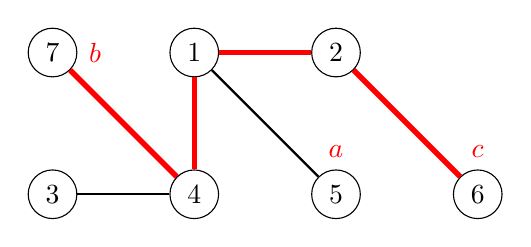
\begin{tikzpicture}[scale=0.9]
\node[draw, circle] (1) at (0,3) {$1$};
\node[draw, circle] (2) at (2,3) {$2$};
\node[draw, circle] (3) at (0,1) {$4$};
\node[draw, circle] (4) at (2,1) {$5$};
\node[draw, circle] (5) at (4,1) {$6$};
\node[draw, circle] (6) at (-2,3) {$7$};
\node[draw, circle] (7) at (-2,1) {$3$};
\path[draw,thick,-] (1) -- (2);
\path[draw,thick,-] (1) -- (3);
\path[draw,thick,-] (1) -- (4);
\path[draw,thick,-] (2) -- (5);
\path[draw,thick,-] (3) -- (6);
\path[draw,thick,-] (3) -- (7);
\node[color=red] at (2,1.6) {$a$};
\node[color=red] at (-1.4,3) {$b$};
\node[color=red] at (4,1.6) {$c$};

\path[draw,thick,-,color=red,line width=2pt] (6) -- (3);
\path[draw,thick,-,color=red,line width=2pt] (3) -- (1);
\path[draw,thick,-,color=red,line width=2pt] (1) -- (2);
\path[draw,thick,-,color=red,line width=2pt] (2) -- (5);
\end{tikzpicture}
\end{center}

This is an elegant method, but why does it work?

It helps to draw the tree differently so that
the path that corresponds to the diameter
is horizontal, and all other
nodes hang from it:
\begin{center}
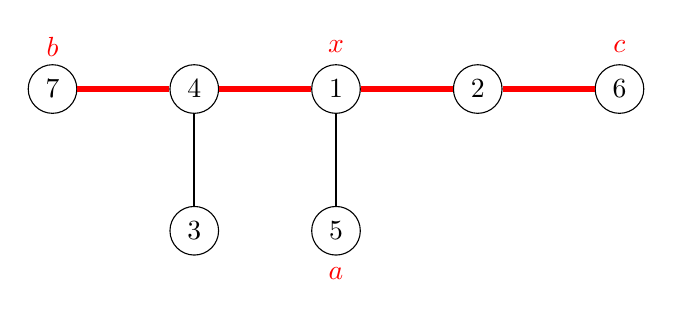
\begin{tikzpicture}[scale=0.9]
\node[draw, circle] (1) at (2,1) {$1$};
\node[draw, circle] (2) at (4,1) {$2$};
\node[draw, circle] (3) at (0,1) {$4$};
\node[draw, circle] (4) at (2,-1) {$5$};
\node[draw, circle] (5) at (6,1) {$6$};
\node[draw, circle] (6) at (0,-1) {$3$};
\node[draw, circle] (7) at (-2,1) {$7$};
\path[draw,thick,-] (1) -- (2);
\path[draw,thick,-] (1) -- (3);
\path[draw,thick,-] (1) -- (4);
\path[draw,thick,-] (2) -- (5);
\path[draw,thick,-] (3) -- (6);
\path[draw,thick,-] (3) -- (7);
\node[color=red] at (2,-1.6) {$a$};
\node[color=red] at (-2,1.6) {$b$};
\node[color=red] at (6,1.6) {$c$};
\node[color=red] at (2,1.6) {$x$};

\path[draw,thick,-,color=red,line width=2pt] (7) -- (3);
\path[draw,thick,-,color=red,line width=2pt] (3) -- (1);
\path[draw,thick,-,color=red,line width=2pt] (1) -- (2);
\path[draw,thick,-,color=red,line width=2pt] (2) -- (5);
\end{tikzpicture}
\end{center}

Node $x$ indicates the place where the path
from node $a$ joins the path that corresponds
to the diameter.
The farthest node from $a$
is node $b$, node $c$ or some other node
that is at least as far from node $x$.
Thus, this node is always a valid choice for
a starting node of a path that corresponds to the diameter.

\section{Distances between nodes}

A more difficult problem is to calculate
for each node in the tree and for each direction,
the maximum distance to a node in that direction.
It turns out that this can be calculated in
$O(n)$ time using dynamic programming.

\begin{samepage}
In the example graph, the distances are as follows:
\begin{center}
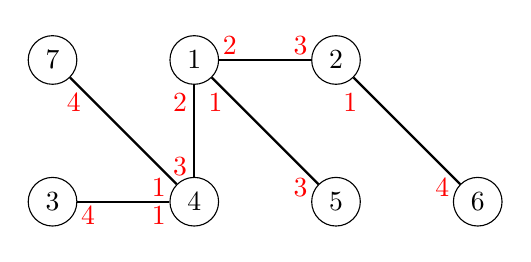
\begin{tikzpicture}[scale=0.9]
\node[draw, circle] (1) at (0,3) {$1$};
\node[draw, circle] (2) at (2,3) {$2$};
\node[draw, circle] (3) at (0,1) {$4$};
\node[draw, circle] (4) at (2,1) {$5$};
\node[draw, circle] (5) at (4,1) {$6$};
\node[draw, circle] (6) at (-2,3) {$7$};
\node[draw, circle] (7) at (-2,1) {$3$};
\path[draw,thick,-] (1) -- (2);
\path[draw,thick,-] (1) -- (3);
\path[draw,thick,-] (1) -- (4);
\path[draw,thick,-] (2) -- (5);
\path[draw,thick,-] (3) -- (6);
\path[draw,thick,-] (3) -- (7);
\node[color=red] at (0.5,3.2) {$2$};
\node[color=red] at (0.3,2.4) {$1$};
\node[color=red] at (-0.2,2.4) {$2$};
\node[color=red] at (-0.2,1.5) {$3$};
\node[color=red] at (-0.5,1.2) {$1$};
\node[color=red] at (-1.7,2.4) {$4$};
\node[color=red] at (-0.5,0.8) {$1$};
\node[color=red] at (-1.5,0.8) {$4$};
\node[color=red] at (1.5,3.2) {$3$};
\node[color=red] at (1.5,1.2) {$3$};
\node[color=red] at (3.5,1.2) {$4$};
\node[color=red] at (2.2,2.4) {$1$};
\end{tikzpicture}
\end{center}
\end{samepage}
For example, the farthest node from node 4
in the direction of node 1 is node 6, and the distance to that
node is 3 using the path
$4 \rightarrow 1 \rightarrow 2 \rightarrow 6$.

\begin{samepage}
Also in this problem, a good starting point
is to root the tree.
After this, all distances to leaves can
be calculated using dynamic programming:
\begin{center}
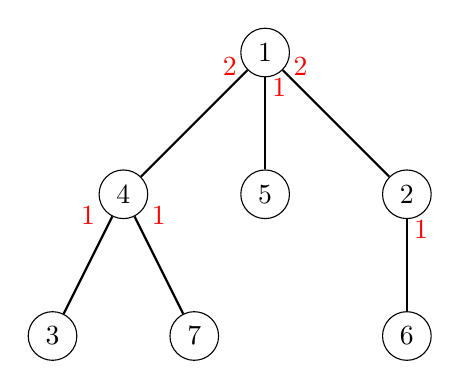
\begin{tikzpicture}[scale=0.9]
\node[draw, circle] (1) at (0,3) {$1$};
\node[draw, circle] (2) at (2,1) {$2$};
\node[draw, circle] (3) at (-2,1) {$4$};
\node[draw, circle] (4) at (0,1) {$5$};
\node[draw, circle] (5) at (2,-1) {$6$};
\node[draw, circle] (6) at (-3,-1) {$3$};
\node[draw, circle] (7) at (-1,-1) {$7$};
\path[draw,thick,-] (1) -- (2);
\path[draw,thick,-] (1) -- (3);
\path[draw,thick,-] (1) -- (4);
\path[draw,thick,-] (2) -- (5);
\path[draw,thick,-] (3) -- (6);
\path[draw,thick,-] (3) -- (7);

\node[color=red] at (-2.5,0.7) {$1$};
\node[color=red] at (-1.5,0.7) {$1$};

\node[color=red] at (2.2,0.5) {$1$};

\node[color=red] at (-0.5,2.8) {$2$};
\node[color=red] at (0.2,2.5) {$1$};
\node[color=red] at (0.5,2.8) {$2$};
\end{tikzpicture}
\end{center}
\end{samepage}

The remaining task is to calculate
the distances through parents.
This can be done by traversing the tree once again
and keeping track of the largest distance from the parent
of the current node to some other node in another direction.

For example, the distance from node 2 upwards
is one larger than the distance from node 1
downwards in some other direction than node 2:
\begin{center}
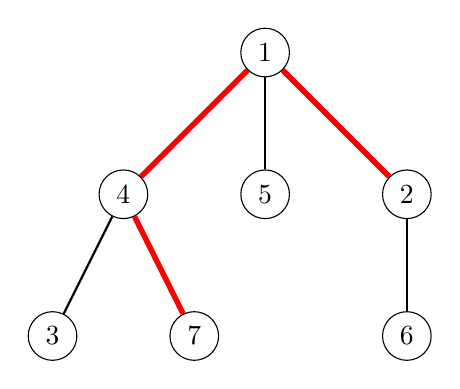
\begin{tikzpicture}[scale=0.9]
\node[draw, circle] (1) at (0,3) {$1$};
\node[draw, circle] (2) at (2,1) {$2$};
\node[draw, circle] (3) at (-2,1) {$4$};
\node[draw, circle] (4) at (0,1) {$5$};
\node[draw, circle] (5) at (2,-1) {$6$};
\node[draw, circle] (6) at (-3,-1) {$3$};
\node[draw, circle] (7) at (-1,-1) {$7$};
\path[draw,thick,-] (1) -- (2);
\path[draw,thick,-] (1) -- (3);
\path[draw,thick,-] (1) -- (4);
\path[draw,thick,-] (2) -- (5);
\path[draw,thick,-] (3) -- (6);
\path[draw,thick,-] (3) -- (7);

\path[draw,thick,-,color=red,line width=2pt] (1) -- (2);
\path[draw,thick,-,color=red,line width=2pt] (1) -- (3);
\path[draw,thick,-,color=red,line width=2pt] (3) -- (7);

\end{tikzpicture}
\end{center}
Finally, we can calculate the distances for all nodes
and all directions:
\begin{center}
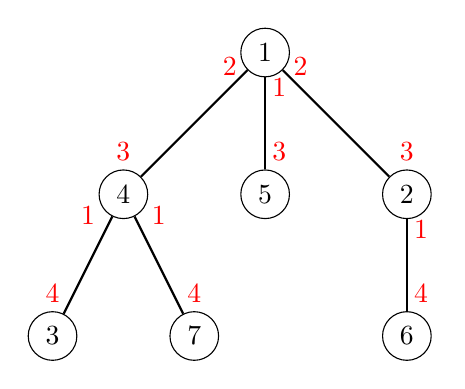
\begin{tikzpicture}[scale=0.9]
\node[draw, circle] (1) at (0,3) {$1$};
\node[draw, circle] (2) at (2,1) {$2$};
\node[draw, circle] (3) at (-2,1) {$4$};
\node[draw, circle] (4) at (0,1) {$5$};
\node[draw, circle] (5) at (2,-1) {$6$};
\node[draw, circle] (6) at (-3,-1) {$3$};
\node[draw, circle] (7) at (-1,-1) {$7$};
\path[draw,thick,-] (1) -- (2);
\path[draw,thick,-] (1) -- (3);
\path[draw,thick,-] (1) -- (4);
\path[draw,thick,-] (2) -- (5);
\path[draw,thick,-] (3) -- (6);
\path[draw,thick,-] (3) -- (7);

\node[color=red] at (-2.5,0.7) {$1$};
\node[color=red] at (-1.5,0.7) {$1$};

\node[color=red] at (2.2,0.5) {$1$};

\node[color=red] at (-0.5,2.8) {$2$};
\node[color=red] at (0.2,2.5) {$1$};
\node[color=red] at (0.5,2.8) {$2$};

\node[color=red] at (-3,-0.4) {$4$};
\node[color=red] at (-1,-0.4) {$4$};
\node[color=red] at (-2,1.6) {$3$};
\node[color=red] at (2,1.6) {$3$};

\node[color=red] at (2.2,-0.4) {$4$};
\node[color=red] at (0.2,1.6) {$3$};
\end{tikzpicture}
\end{center}

\section{Binary trees}

\index{binary tree}

\begin{samepage}
A \key{binary tree} is a rooted tree
where each node has a left and right subtree.
It is possible that a subtree of a node is empty.
Thus, every node in a binary tree has
zero, one or two children.

For example, the following tree is a binary tree:
\begin{center}
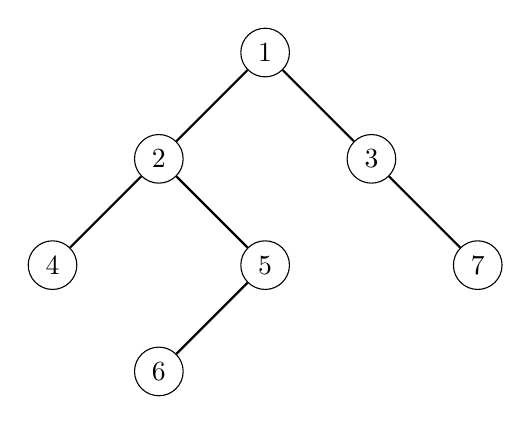
\begin{tikzpicture}[scale=0.9]
\node[draw, circle] (1) at (0,0) {$1$};
\node[draw, circle] (2) at (-1.5,-1.5) {$2$};
\node[draw, circle] (3) at (1.5,-1.5) {$3$};
\node[draw, circle] (4) at (-3,-3) {$4$};
\node[draw, circle] (5) at (0,-3) {$5$};
\node[draw, circle] (6) at (-1.5,-4.5) {$6$};
\node[draw, circle] (7) at (3,-3) {$7$};

\path[draw,thick,-] (1) -- (2);
\path[draw,thick,-] (1) -- (3);
\path[draw,thick,-] (2) -- (4);
\path[draw,thick,-] (2) -- (5);
\path[draw,thick,-] (5) -- (6);
\path[draw,thick,-] (3) -- (7);
\end{tikzpicture}
\end{center}
\end{samepage}

\index{pre-order}
\index{in-order}
\index{post-order}

The nodes in a binary tree have three natural
orderings that correspond to different ways to 
recursively traverse the tree:

\begin{itemize}
\item \key{pre-order}: first process the root,
then traverse the left subtree, then traverse the right subtree
\item \key{in-order}: first traverse the left subtree,
then process the root, then traverse the right subtree
\item \key{post-order}: first traverse the left subtree,
then traverse the right subtree, then process the root
\end{itemize}

For the above tree, the nodes in
pre-order are
$[1,2,4,5,6,3,7]$,
in in-order $[4,2,6,5,1,3,7]$
and in post-order $[4,6,5,2,7,3,1]$.

If we know the pre-order and in-order
of a tree, we can reconstruct the exact structure of the tree.
For example, the above tree is the only possible tree
with pre-order $[1,2,4,5,6,3,7]$ and
in-order $[4,2,6,5,1,3,7]$.
In a similar way, the post-order and in-order
also determine the structure of a tree.

However, the situation is different if we only know
the pre-order and post-order of a tree.
In this case, there may be more than one tree
that match the orderings.
For example, in both of the trees
\begin{center}
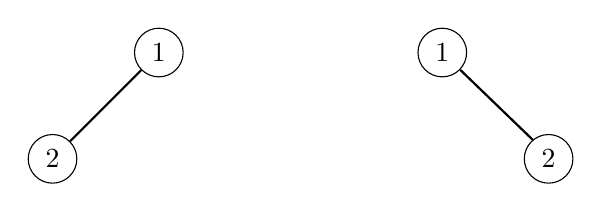
\begin{tikzpicture}[scale=0.9]
\node[draw, circle] (1) at (0,0) {$1$};
\node[draw, circle] (2) at (-1.5,-1.5) {$2$};
\path[draw,thick,-] (1) -- (2);

\node[draw, circle] (1b) at (0+4,0) {$1$};
\node[draw, circle] (2b) at (1.5+4,-1.5) {$2$};
\path[draw,thick,-] (1b) -- (2b);
\end{tikzpicture}
\end{center}
the pre-order is $[1,2]$ and the post-order is $[2,1]$,
but the structures of the trees are different.

